\documentclass{article}
\usepackage{graphicx}
\usepackage[export]{adjustbox}

\title{Homework 2 CSCI 451}
\author{Nicholas Rust}
\date{due: 27 September 2019}

\begin{document}
\maketitle

\section{Exercise 2 (textbook section 2.7, pg 54)}
A dynamic programming solution to find the longest common subsequence between two strings could be to make a matrix of the two strings, similar to how we have implimented global alignment. Effectively, using Needleman-Wunsch slightly modified would work well to find the longest common subsequence.

\section{Exercise 3 (textbook section 2.7, pg 54)}
a.
\begin{verbatim}
Match: 2
mismatch: -1
deletion/insertion: -1

S = A/CAATCG
T = CTCATG/C

Global Alignment (G):
ACAATC-G-
-C--TCAGC

Local Alignment (L):
CAATCG
C-AT-G

Global Alignment without first of S or last of T (H):
CAATC--G
C--TCATG

Global alignment score: 3 (8-5)

Local alignment score: 6 (8-2)

Global without first/last: 4 (8-4)
\end{verbatim}

b. Given the nature of local alignment for any two strings S and T that are to be compared, the local alignment will never have a score worse than the global. Since local alignments are able to pick the best portion of the two strings to match, and given that the global has a score X, and that the local alignment will include the portion with the best alignment, then the local alignment will also be greater than or equal to the global alignment.

However, I do believe that the global alignment without the first character of S and the last character of T can have a lower score than the global alignment.
\begin{verbatim}
Example:

Match: 2
mismatch: -1
deletion/insertion: -1

Global

S = CAAAAAAAC
T = CTTTTTTTC

score = -3 (4-7)

Then chop of the required letters:

Global missing letters

S = AAAAAAAC
T = CTTTTTTT 

score = -8 (0 - 8)
\end{verbatim}

\begin{figure}
	\section{Global Alignment}
    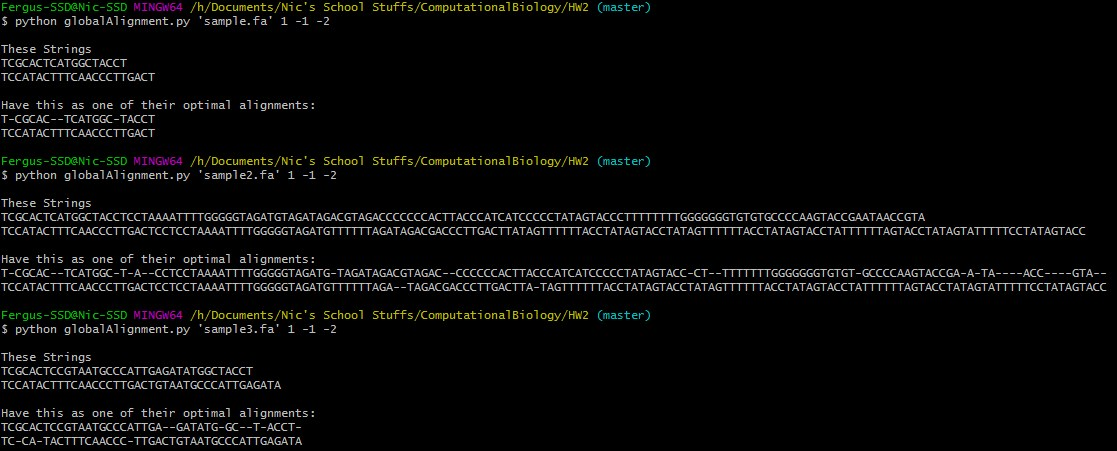
\includegraphics[width=1.75\textwidth,center]{HW2Output.jpg}
    \caption{Program Output}
\end{figure}

\end{document}